\documentclass{article}

\usepackage[a4paper, top=2cm, bottom=3cm]{geometry}

\usepackage[ngerman]{babel}
\usepackage{csquotes}

\usepackage{booktabs}
\usepackage{mathtools}
\usepackage{amssymb}
\usepackage{enumitem}
\usepackage{amsmath}

\usepackage{hyperref}

\usepackage{graphicx}
\usepackage{wrapfig}

\usepackage{pgfplots}
\pgfplotsset{compat=1.18}

\usepackage{siunitx}
\sisetup{locale = DE}
\usepackage[version=4]{mhchem}

\usepackage{biblatex}
\DefineBibliographyStrings{ngerman}{
  urlseen = {Abruf vom}
}
\addbibresource{quellen.bib}

\newcommand{\proofeq}{\overset{!}{=}}
\newcommand{\proofeqv}{\overset{!}{\Leftrightarrow}}
\newcommand{\equivalent}{\overset{\scriptscriptstyle\wedge}{=}}
\DeclarePairedDelimiter\ceil{\lceil}{\rceil}
\DeclarePairedDelimiter\floor{\lfloor}{\rfloor}

\date{24.03.2022}
\title{Physikalisches Grundpraktikum Teil I \\ (Mechanik und Thermodynamik) \\ Versuch 5: Luftballon mit \ce{CO2}}
\author{Wafaa Al Nachwati; Matrikelnummer: 8102531 \\ Finn Wagner; Matrikelnummer: 8102237}

\begin{document}

    \maketitle

    \section{Versuchsziel und Versuchsmethode}
      In diesem Versuch wird die Dichte von \ce{CO2} über die Fallzeit eines mit \ce{CO2} gefüllten Luftballons bestimmt.
      Der Fall des Luftballons wird als Bewegung eines kugelförmigen Körpers in einer Flüssigkeit (Luft oder Luft als Quasi-Flüssigkeit) mit laminarer Strömung approximiert.

    \section{Grundlagen}
      Wir füllen zwei Luftballons, einmal mit Luft und einmal mit \ce{CO2}. Auf beide Luftballons wirkt die gleiche Auftriebskraft, da sie das gleiche Volumen an Luft verdrängen.
      Aber, da sich ihre Massen unterscheiden wirkt auf den mit \ce{CO2} gefüllten Luftballon, wie wir später sehen werden, aufgrund der höheren Dichte von \ce{CO2}
      eine stärkere Gewichtskraft, die mehr von der geschwindigkeitsabhängigen Reibungskraft überwinden kann. Der mit \ce{CO2} gefüllte Luftballon fällt schneller.
      Aus dieser Beziehung zwischen Dichte und Geschwindigkeit stellen wir eine Formel auf und können durch Messen des Volumens der Luftballons, sowie der Fallgeschwindigkeiten
      zunächst den Faktor zwischen den beiden Dichten und da wir die Dichte von Luft bereits kennen~\cite{Aufgabenstellung}, die Dichte von \ce{CO2} berechnen.

    \section{Formeln}
      Auf jeden Körper wirkt im Schwerefeld der Erde eine Zentralkraft Richtung Erdmittelpunkt, proportional zur Masse des Körpers.
      \begin{equation} \label{eq:schwerkraft}
          F_G = m \cdot g
      \end{equation}
      Die Masse eines Körpers (mit Dichte \(\rho_K\)) können wir auch über seine Dichte und sein Volumen ausdrücken mit der Beziehung:
      \begin{equation} \label{eq:masse_dichte_rel}
          m = \rho_K \cdot V
      \end{equation}
      Weiterhin wirkt auf Körper mit echter Ausdehnung (keine Punktmasse) in Flüssigkeiten/Gasen wie Luft eine Auftriebskraft,
      die durch Verdrängung des Mediums entsteht. Sie ist abhängig vom verdrängten Volumen und der Dichte des Mediums (Gases \(\rho_G\)) in dem sich der Körper befindet.
      \begin{equation} \label{eq:auftrieb}
          F_A = \rho_{G} \cdot V \cdot g
      \end{equation}
      Als dritte Kraft wirkt bei unserem Versuch eine Reibungskraft gegen den Fall des Luftballons an.
      Die stokessche Reibung ist proportional zur Geschwindigkeit \(v\), dem Radius \(r\) des Luftballons, so wie der Viskosität \( \eta \) der Luft.
      \begin{equation} \label{eq:stokes_reibung}
          F_R = 6 \pi \cdot r \cdot \eta \cdot v
      \end{equation}
      Wir setzen hier stokessche Reibung an, da wir uns vollständig im Bereich laminarer Strömung aufgrund sehr kleiner Geschwindigkeiten befinden.
      Der Luftballon wird als von der Schwerkraft nach unten beschleunigt, vom Auftrieb und von der Reibungskraft gebremst.
      Der Luftballon beschleunigt bis zu seiner maximalen Fallgeschwindigkeit (Siehe~\cite{Fall-Luftwiederstand}) und fällt ab dann mit einer konstanten Geschwindigkeit weiter,
      wird also nicht mehr weiter beschleunigt, da auf den Ballon keine resultierende Kraft mehr wirkt (Gleichung~\ref{eq:gleichgewicht}).
      Da für unsere Gegebenheiten die Zeit in der der Luftballon beschleunigt im Vergleich zur gesamten Fallzeit sehr gering ist,
      setzen wir für den gesamten Fall das Kräftegleichgewicht an, tun also so, als ob der Ballon direkt mit seiner Endgeschwindigkeit fällt:
      \begin{equation} \label{eq:gleichgewicht}
          F_G = F_A + F_R
      \end{equation}
      Wir approximieren also, dass der Luftballon auf der gesamten Strecke \(h\) mit der selben Geschwindigkeit \(v\) fällt. Er braucht dazu die Zeit \(t_{Fall}\)
      \begin{equation} \label{eq:geschwindigkeit}
          v = \frac{h}{t_{Fall}}
      \end{equation}
      Die Endgeschwindigkeit des Ballons lässt sich aus dem Kräftegleichgewicht (Formel~\ref{eq:gleichgewicht}) durch Einsetzen der stokesschen Reibung ausdrücken:
      \begin{equation}
          \begin{gathered} \label{eq:stokes_geschwindigkeit}
              F_G = F_A + F_R \Rightarrow F_R = F_G - F_A \\
              \Rightarrow 6 \pi \cdot r \cdot \eta \cdot v = F_G - F_A \\
              \Rightarrow v = \frac{ F_G - F_A }{ 6 \pi \cdot r \cdot \eta }
          \end{gathered}
      \end{equation}
      Wir setzen nun Gleichung~(\ref{eq:geschwindigkeit}) und Gleichung~(\ref{eq:stokes_geschwindigkeit}) gleich.
      \begin{equation} \label{eq:fall_halb}
          \frac{h}{t_{Fall}} = \frac{ F_G - F_A }{ 6 \pi \cdot r \cdot \eta }
      \end{equation}
      Im Experiment werden zwei Luftballons, einer gefüllt mit \ce{CO2} und einer gefüllt mit Luft, aus der selben Höhe \(h\) fallengelassen.
      Die Masse m eines solchen gefüllten Luftballons setzt sich aus der Masse \( m_h \) des Ballons (der Ballonhülle aus Gummi), sowie dem in ihm enthaltenen Gas (Formel~\ref{eq:masse_dichte_rel}) zusammen.
      Wir setzen diese Masse in die Formel für die Schwerkraft\ref{eq:schwerkraft} ein:
      \begin{equation} \label{eq:schwerkraft_ballon}
          F_G = m \cdot g = m_H \cdot g + \rho \cdot V \cdot g = \left( m_H + \rho \cdot V \right) \cdot g
      \end{equation}
      Die Schwerkraft (Formel~\ref{eq:schwerkraft_ballon}), sowie die Auftriebskraft (Formel~\ref{eq:auftrieb}) setzen wir in Gleichung~\ref{eq:fall_halb} ein:
      \begin{equation} \label{eq:fall}
          \frac{h}{t_{Fall}} = \frac{ \left( m_H + \rho_{F\ddot{u}llung} \cdot V \right) \cdot g - \rho_{Medium} \cdot V \cdot g }{ 6 \pi \cdot r \cdot \eta_{Medium} }
      \end{equation}
      Zu unterscheiden sind die beiden Dichten. \(\rho_{F\ddot{u}llung}\) ist die Dichte des Gases im Luftballon, \(\rho_{Medium}\) die Dichte des Gases in der Atmosphäre.
      Für den Luftballon gefüllt mit Luft wird Formel~\ref{eq:fall} zu:
      \begin{equation} \label{eq:fall_luft}
          \frac{h}{t_{Luft}} = \frac{ \left( m_H + \rho_{Luft} \cdot V \right) \cdot g - \rho_{Luft} \cdot V \cdot g }{ 6 \pi \cdot r \cdot \eta_{Luft} }
      \end{equation}
      Und für den Luftballon gefüllt mit \ce{CO2} wird Formel~\ref{eq:fall} zu:
      \begin{equation} \label{eq:fall_co2}
          \frac{h}{t_{\ce{CO2}}} = \frac{ \left( m_H + \rho_{\ce{CO2}} \cdot V \right) \cdot g - \rho_{Luft} \cdot V \cdot g }{ 6 \pi \cdot r \cdot \eta_{Luft} }
      \end{equation}
      Wir teilen nun die Formel für den Fall in \ce{CO2} durch die für den Fall in Luft und vereinfachen:
      \begin{equation} \label{eq:calc_rho_faktor}
          \begin{gathered}
              \frac{ \frac{h}{t_{\ce{CO2}}} }{ \frac{h}{t_{Luft}} } = \frac{ t_{Luft} }{ t_{\ce{CO2}} } =
              \frac{ \frac{ \left( m_H + \rho_{\ce{CO2}} \cdot V \right) \cdot g - \rho_{Luft} \cdot V \cdot g }{ 6 \pi \cdot r \cdot \eta_{Luft} } }
              { \frac{ \left( m_H + \rho_{Luft} \cdot V \right) \cdot g - \rho_{Luft} \cdot V \cdot g }{ 6 \pi \cdot r \cdot \eta_{Luft} } } = \\
              \frac{ \left( m_H + \rho_{\ce{CO2}} \cdot V \right) \cdot g - \rho_{Luft} \cdot V \cdot g }{ \left( m_H + \rho_{Luft} \cdot V \right) \cdot g - \rho_{Luft} \cdot V \cdot g } =
              \frac{ \left( m_H + \rho_{\ce{CO2}} \cdot V \right) \cdot g - \rho_{Luft} \cdot V \cdot g }{ m_H \cdot g + \left( \rho_{Luft} \cdot V \cdot g - \rho_{Luft} \cdot V \cdot g \right) } = \\
              \frac{ \left( m_H + \rho_{\ce{CO2}} \cdot V \right) - \rho_{Luft} \cdot V }{ m_H } = \\
              \frac{ m_H + V \cdot \left( \rho_{\ce{CO2}} - \rho_{Luft} \right)}{ m_H } = 1 + \frac{V}{m_H} \left( \rho_{\ce{CO2}} - \rho_{Luft} \right)
          \end{gathered}
      \end{equation}
      Im letzten Schritt formen wir noch nach \(\rho_{\ce{CO2}}\) um:
      \begin{equation} \label{eq:calc_rho_co2}
          \rho_{\ce{CO2}} = \rho_{Luft} + \left( \frac{t_{Luft}}{t_{\ce{CO2}}} - 1 \right) \frac{m_H}{V}
      \end{equation}

    \section{Versuchsaufbau}
      \begin{figure}[ht]
          \centering
          \begin{minipage}[t]{0.4\textwidth}\label{fig:versuch_schematik}
              \includegraphics[height=6cm]{kräfte.png}
              \caption{Schematische Darstellung des Versuchs und der auftretenden Kräfte}
          \end{minipage}
          \hfill
          \begin{minipage}[t]{0.4\textwidth}\label{fig:abmessungen}
              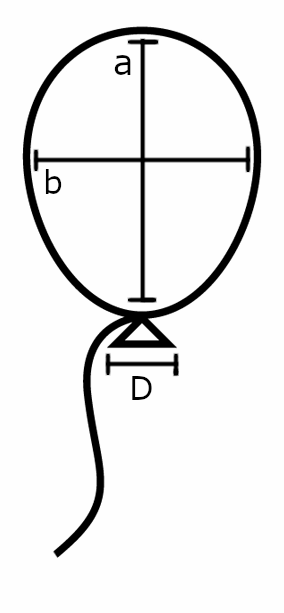
\includegraphics[height=6cm]{luftballons.png}
              \caption{Messgrößen am Luftballon}
          \end{minipage}
      \end{figure}

      \subsection{Material}
          \begin{itemize}
              \item 2 Luftballons
              \item 1 Flasche Mineralwasser Classic; Wasser mit viel Kohlensäure
              \item Smartphone zum Aufnehmen eines Videos
              \item Maßband mit mindestens Millimetergenauigkeit, am besten ein weiches Rollbandmaß
              \item 1 Stoppuhr oder Computerprogramm zum Auswerten der Zeiten im Video
          \end{itemize}

    \section{Durchführung}
      \subsection{Ballon mit \texorpdfstring{\ce{CO2}}{CO2} aufpumpen}
          \begin{enumerate}
              \item Stülpen Sie den Luftballon (d.h.\ das Mundstück des Luftballons) auf den Hals der Mineralwasserflasche
              \item Schütteln Sie die Wasserflasche wiederholt, um die im Wasser gelöste Kohlensäure in \ce{CO2}-Gas umzuwandeln und den Luftballon dadurch aufzublasen.
                    Achten Sie darauf, dass kein Wasser in den Ballon kommt, um die Masse des Ballons nicht zu verändern.
              \item Der Ballon muss am Ende nicht vollständig aufgeblasen sein; etwa \(\SI{15}{cm}\) sind bereits ausreichend.
              \item Halten sie den Ballon zu und nehmen sie ihn vorsichtig von der Flasche, sodass kein \ce{CO2} entweicht und knoten Sie ihn zu.
          \end{enumerate}

      \subsection{Zweiten Ballon füllen}
          \begin{enumerate}[resume]
              \item Bestimmen Sie die Umfänge des mit \ce{CO2} gefüllten Ballons mithilfe des Maßbands.
                    Messen Sie den Umfang vom Mundstück bis zum obersten Punkt (Umfang a), sowie die \enquote{Taille} (Umfang b) (Siehe~\ref{fig:abmessungen})
              \item Pusten Sie einen zweiten Ballon (mit Luft) auf. Lassen sie in kleinen Schritten Luft aus dem Ballon und messen Sie wiederholt die Umfänge,
                    bis die beiden Luftballons ein identisches Volumen haben.
              \item Knoten Sie den Luftballon zu.
          \end{enumerate}

      \subsection{Fallversuch}
          \begin{enumerate}[resume]
              \item Suchen Sie sich einen Ort als Referenzpunkt in gut 2 Metern Höhe (z.B.\ Oberkante eines Schranks, Türrahmen) und messen Sie
                    den Abstand \(h\) zum Boden.
              \item Starten Sie ein Video auf ihrem Handy mit Stativ oder lassen Sie sich von einer zweiten Person helfen.
                    Nehmen Sie das Video von etwas weiter weg auf und achten Sie darauf das der Start, sowie das Aufkommen auf dem Boden im Video gut zu sehen sind.
              \item Halten Sie die beiden Luftballons in Höhe \(h\) und lassen Sie sie gleichzeitig fallen. Wie in Bild~\ref{fig:Fall2} gezeigt.
              \item Wiederholen Sie den Fallversuch 3 mal, nehmen Sie also 2 weitere Videos auf.
          \end{enumerate}

      \subsection{Videoauswertung}
          \begin{enumerate}
              \item Messen Sie bei allen aufgenommen Videos die Fallzeiten der Luftballons vom Zeitpunkt an dem sie losgelassen wurden, bis sie auf den Boden aufkommen.
                    Dies kann durch mitstoppen mit einer Stoppuhr beim anschauen des Videos oder durch direktes auswerten des Videos mit Hilfe eines geeigneten Computerprogramms oder Handyapp.
          \end{enumerate}

    \section{Messergebnisse}
      Für die drei Messungen haben wir die folgenden Werte aufgenommen: \\
      \begin{center}
          \begin{tabular}{|c|c|c|}
              \hline
                        & \( t_{\ce{co2}} [s] \) & \( t_{Luft} [s] \) \\
              \hline
              \( t_1 \) & 1,195                  & 1,542 \\
              \hline
              \( t_2 \) & 1,251                  & 1,528 \\
              \hline
              \( t_3 \) & 1,306                  & 1,515 \\
              \hline
          \end{tabular} \\
      \end{center}
      Für die Umfänge der Luftballons haben wir folgende Werte gemessen:
      \( a = \SI{47.5}{cm} = \SI{0.475}{\metre} \) und \( b = \SI{45}{cm} = \SI{0.45}{\metre} \) für den ersten, mit \ce{CO2} gefüllten Luftballon und
      \( a = \SI{47.7}{cm} = \SI{0.477}{\metre} \) und \( b = \SI{45}{cm} = \SI{0.45}{\metre} \) für den zweiten mit Luft gefüllten Luftballon.
      Die Luftballons wurden von einer Höhe von \( h = \SI{1.97}{\metre} \) fallen gelassen. \\
      Zusätzlich haben wir die Masse der von uns verwendeten Luftballons mit einer sehr genauen Waage auf
      \( m_H = \SI{2}{\gram} \) bestimmt, wir rechen aber trotzdem mit \( m_H = \SI{5}{\gram}\)

    \section{Auswertung}
      Aus den gemessenen Fallzeiten berechnen wir die durchschnittlichen Fallzeiten für die beiden Luftballons: \\
      \begin{equation}\label{eq:mittel_coo}
          \overline{t_{\ce{co2}}} = \frac{ \SI{1,195}{\second} + \SI{1,251}{\second} + \SI{1,306}{\second} }{3} \approx \SI{1.251}{\second} % (1.195 + 1.251 + 1.306 )/3    
      \end{equation}
      \begin{equation}
          \overline{t_{Luft}} = \frac{ \SI{1,542}{\second} + \SI{1,528}{\second} + \SI{1,515}{\second} }{3} \approx \SI{1.528}{\second} % (1.542 + 1.528 + 1.515 )/3    
      \end{equation}
      Für unsere Rechnungen nehmen wir an, dass die Luftballons das gleiche Volumen haben.
      Wir rechnen demnach aus all unseren Messungen einen repräsentativen mittleren Umfang aus:
      \begin{equation}
          \begin{gathered}
              \bar{a} = \frac{ \SI{0.475}{\metre} + \SI{0.477}{\metre} }{2} = \SI{0.476}{\metre} \\
              \Rightarrow U = \frac{ \SI{0.476}{m} + \SI{0.45}{m} }{2} = \SI{0.463}{m}
          \end{gathered}
      \end{equation}
      Wir berechnen das Volumen des Luftballons mit der Annahme, dass der Luftballon ein kugelförmiger Körper ist und das Mundstück nicht zum Volumen des Luftballons dazu zählt:
      \begin{equation}\label{eq:volumen}
          \begin{gathered}
              V = \frac{4}{3} \pi {\left( \frac{U}{2 \pi} \right) }^3 = \frac{4}{3} \pi \frac{U^3}{8 \pi^3} = \frac{1}{6} \frac{U^3}{\pi^2} \\
              V = \frac{ {( \SI{0.463}{\metre} )}^3 }{ 6 \cdot \pi^2} = \SI{1.676e-3}{m^3}
          \end{gathered}
      \end{equation}
      Für die Dichte ergibt also:
      Wir setzen die Dichte von Luft \( \rho_{Luft} = \SI{1.2041}{ \frac{\kilogram}{\metre^3} } \)(Wert aus~\cite{Aufgabenstellung}), die Masse des Luftballons \(m_H = \SI{5}{\gram} = \SI{0,005}{\kilogram} \),
      das berechnete Volumen \(V = \SI{1.676e-3}{m^3} \), sowie die Mittelwerte der gemessenen Fallzeiten in Formel~(\ref{eq:calc_rho_co2}) ein:
      \begin{equation}
          \begin{gathered}
              \rho_{\ce{CO2}} = \rho_{Luft} + \left( \frac{t_{Luft}}{t_{\ce{CO2}}} - 1 \right) \frac{m_H}{V} \\
              \Rightarrow \rho_{\ce{CO2}} = \SI{ 1,2041 }{ \frac{kg}{m^3} } + \left( \frac{ \SI{1,528}{s} }{ \SI{1,251}{s} } - 1 \right) \cdot \frac{ \SI{0,005}{\kilogram} }{ \SI{0,001676}{m^3} } \\
              \Rightarrow \rho_{\ce{CO2}} \approx \SI{1.8647}{\frac{kg}{m^3}}
          \end{gathered}
      \end{equation}
      \subsection{Fehlerrechnung}

          \subsubsection{Fehler der Zeitmessungen}
              Für die Fehlerrechnung wird die Standardabweichung des Mittelwertes berechnet. Wir verwenden dafür die Formel aus~\cite{AnleitungPraktikum} (0.2.1.7)
              \begin{equation}
                  \begin{gathered}
                      \sigma( \overline{t} ) = \frac{1}{\sqrt{N}} \sigma(\overline{t}) \\
                      \approx \sqrt{ \frac{1}{ N (N-1) } \left( {(t_1 - \overline{t})}^2 + {( t_2 - \overline{t} )}^2 + {( t_3 - \overline{t} )}^2 \right) } \\
                  \end{gathered}
              \end{equation}
              Für die Fallzeiten mit \ce{CO2}:
              \begin{equation}
                  \begin{gathered}
                      \sigma(\overline{t_{co2}})=
                      \sqrt{ \frac{1}{6} \left( {( \SI{1,195}{s} - \SI{1,251}{s} )}^2 + {( \SI{1,251}{s} - \SI{1,251}{s} )}^2 + {( \SI{1,306}{s} - \SI{1,251}{s} )}^2 \right) } \\
                      \approx 0,032s
                  \end{gathered}
              \end{equation}
              Für die Fallzeiten mit Luft:
              \begin{equation}
                  \begin{gathered}
                      \sigma(\overline{t_{Luft}}) =
                      \sqrt{ \frac{1}{6} \left( {( \SI{1,542}{s} - \SI{1,528}{s} )}^2 + {( \SI{1,528}{s} - \SI{1,528}{s} )}^2 + {( \SI{1,515}{s} - \SI{1,528}{s} )}^2 \right) } \\
                      \approx 0,007s
                  \end{gathered}
              \end{equation}

          \subsubsection{Fehlerfortpflanzung}
              Wir setzen zunächst die Formel für das Volumen~(\ref{eq:volumen}) in die Formel zur Berechnung der Dichte~(\ref{eq:calc_rho_co2}) ein:
              \begin{equation}
                  \rho_{\ce{CO2}} = \rho_{Luft} + \left( \frac{t_{Luft}}{t_{\ce{CO2}}} - 1 \right) \frac{m_H}{V}\\
                  = \rho_{Luft} + \left( \frac{t_{Luft}}{t_{\ce{CO2}}} - 1 \right) \frac{m_H}{\frac{1}{6} \frac{U^3}{\pi^2}}
              \end{equation}
              Wir berechnen nun den Fehler der Dichte über Fehlerfortpflanzung:
              \begin{equation}
                  \Delta \rho_{\ce{CO2}} = \sqrt{
                  {\left( \frac{ \partial \rho_{\ce{CO2}} }{ \partial t_{Luft} } \cdot \Delta t_{Luft} \right)}^2 +
                  {\left( \frac{ \partial \rho_{CO2} }{ \partial t_{\ce{CO2}} } \cdot \Delta t_{\ce{CO2}} \right)}^2 +
                  {\left( \frac{ \partial \rho_{CO2} }{ \partial U } \cdot \Delta U \right)}^2
                  }
              \end{equation}
              Wir berechnen die partiellen Ableitungen:
              \begin{equation}
                  \begin{aligned}
                      \frac{ \partial \rho_{\ce{CO2}} }{ \partial t_{Luft} }     & = \frac{ \partial }{ \partial t_{Luft} }     \left( \rho_{Luft} + \left( \frac{t_{Luft}}{t_{\ce{CO2}}} - 1 \right) \frac{m_H}{\frac{1}{6} \frac{U^3}{\pi^2}} \right) = \frac{6 \cdot \pi^2 \cdot m}{t_{\ce{CO2}} \cdot U^3}                                  \\
                      \frac{ \partial \rho_{\ce{CO2}} }{ \partial t_{\ce{CO2}} } & = \frac{ \partial }{ \partial t_{\ce{CO2}} } \left( \rho_{Luft} + \left( \frac{t_{Luft}}{t_{\ce{CO2}}} - 1 \right) \frac{m_H}{\frac{1}{6} \frac{U^3}{\pi^2}} \right) = -\frac{6 \pi^2 \cdot t_{Luft} \cdot m }{ t_{\ce{CO2}}^2 \cdot U^3 }                   \\
                      \frac{ \partial \rho_{\ce{CO2}} }{ \partial U }            & = \frac{ \partial }{ \partial U }            \left( \rho_{Luft} + \left( \frac{t_{Luft}}{t_{\ce{CO2}}} - 1 \right) \frac{m_H}{\frac{1}{6} \frac{U^3}{\pi^2}} \right) = \frac{ 18 \pi^2 \cdot m \cdot ( t_{\ce{CO2}} - t_{Luft} ) }{ t_{\ce{CO2}} \cdot U^4 }
                  \end{aligned}
              \end{equation}
              Einsetzen:
              \begin{equation}
                  \begin{gathered}
                      \Delta \rho_{\ce{CO2}} =
                      \sqrt{ { \left( \frac{ 6 \cdot \pi^2 \cdot m }{ t_{\ce{CO2}} \cdot U^3 } \cdot \Delta t_{Luft} \right) }^2 + } \\
                      \overline{ { \left( -\frac{ 6 \pi^2 \cdot t_{Luft} \cdot m }{ t_{\ce{CO2}}^2 \cdot U^3 } \cdot \Delta t_{\ce{CO2}} \right)}^2 + }
                      \overline{ { \left( \frac{ 18 \pi^2 \cdot m \cdot ( t_{\ce{CO2}} - t_{Luft} ) }{ t_{\ce{CO2}} \cdot U^4 } \cdot \Delta U \right)}^2 }
                  \end{gathered}
              \end{equation}
              Wir setzen die Masse des Luftballons \(m = \SI{0.005}{\kilogram}\), den Umfang \( U = \SI{0.463}{m} \),
              sowie die beiden durchschnittlichen Zeiten \( \overline{t_{\ce{co2}}} = \SI{1.251}{\second} \) und \(\overline{t_{Luft}} = \SI{1.528}{\second} \) ein.
              Für die Zeitunsicherheiten setzen wir die Standardabweichung ein, also \( \Delta t_{Luft} = \SI{0.007}{s} \) und \( \Delta t_{\ce{CO2}} = \SI{0.032}{s} \).
              Für die Unsicherheit des Umfangs setzen wir \( \Delta U = \SI{0.009}{m} \) an,
              diesen Wert haben wir als Standardabweichung von 6 Messungen am gleichen Luftballon durchgeführten Messungen berechnet.
              \begin{equation}
                  \begin{aligned}
                      \Delta \rho_{\ce{CO2}} & =                                                                                                                                                                              \\
                                             & \sqrt{ { \left( \frac{6 \cdot \pi^2 \cdot \SI{0.005}{kg} }{ \SI{1.251}{s} \cdot {(\SI{0.463}{m})}^3 } \cdot \SI{0.007}{s} \right)}^2 +}                                        \\
                                             & \overline{ { \left( -\frac{6 \pi^2 \cdot \SI{1.528}{s} \cdot \SI{0.005}{kg} }{ {(\SI{1.251}{s})}^2 \cdot {(\SI{0.463}{m})}^3 } \cdot \SI{0.032}{s} \right)}^2 + }              \\
                                             & \overline{ { \left( \frac{ 18 \pi^2 \cdot \SI{0.005}{kg} \cdot ( \SI{1.251}{s} - \SI{1.528}{s} ) }{ \SI{1.251}{s} \cdot {(\SI{0.463}{m})}^4 } \cdot \SI{0.009}{m} \right)}^2 } \\
                      \approx \SI{0.102}{\frac{kg}{m^3}}
                  \end{aligned}
              \end{equation}
              % sqrt( (6*pi^2*0.005kg /(1.251s*(0.463m)^3) * 0.007s)^2 + (-6*pi^2*1.528s*0.005kg/((1.251s)^2*(0.463m)^3)*0.032s)^2 + (18*pi^2*0.005kg*(1.251s-1.528s)/(1.251s*(0.463m)^4)*0.009m)^2 )

      \subsection{Endergebnis}
          Wir kommen also am Ende auf:
          \begin{equation}
              \SI{1.87}{\frac{kg}{m^3}} \pm \SI{0.1}{\frac{kg}{m^3}}
          \end{equation}
          Der Literaturwert der Dichte von Kohlenstoffdioxid \( \ce{CO2} \) bei Atmosphärendruck \(\SI{1.01325 }{bar}\) und Raumtemperatur von \(\SI{20}{\celsius}\) ist \( \SI{1,8393}{ \frac{ \kilogram }{ \metre^3 } } \)
          (Aus Quelle~\cite{co2dichteneu}) \\
          Wir berechnen nun die Abweichung unseres berechneten Wertes von einem Literaturwert von \ce{CO2}:
          \begin{equation}
              \frac{ \rho_{Literatur}}{\rho_{Experiment}} = \left( 1 - \frac{ \SI{ 1,8393 }{ \frac{kg}{m^3} } }{ \SI{1,865}{ \frac{kg}{m^3} } } \right) \cdot 100 = 1,6 \%
          \end{equation}
          Also eine Abweichung von ungefähr 1,6 \%.
    \section{Fall auf der Venus}
      Wir bestimmen nun, wie lang der Fall des mit \ce{CO2} gefüllten Luftballons auf der Venus dauern würde, aus der gleichen Höhe zu Boden zu fallen. Wir nehmen an,
      dass die Atmosphäre der Venus zu \( 100\% \) aus \ce{CO2} besteht. Die Schwerkraft auf der Venus beträgt \(g_{Venus} = \SI{8.87}{\frac{m}{s}}\).
      Die Atmosphäre auf der Venus ist mit mehr als \(\SI{400}{\celsius}\) sehr heiß und die Viskosität ist abhängig von der Temperatur.
      Wir nehmen für diese Rechnung an, dass es auf der Venus nur Raumtemperatur mit \(T = \SI{20}{\celsius}\) warm ist.
      Die Viskosität von \ce{CO2} ist dann \( \eta_{\ce{CO2}} = \SI{14.73e-6}{\pascal\cdot\second} \).
      Um die Zeit zu berechnen stellen wir zwei Ansätze vor. \\

      \subsection{Ansatz 1}
          Wir berechnen die Geschwindigkeit mithilfe der hergeleiteten Formel~(\ref{eq:stokes_geschwindigkeit}) im Theorieteil.
          \begin{equation}\label{eq:fall_venus}
              \begin{gathered}
                  v = \frac{ F_G - F_A }{ 6 \pi \cdot r \cdot \eta } \\
                  v= \frac{m_H \cdot g_{Venus}+\rho_{co2}\cdot V \cdot g_{Venus} - \rho_{co2}\cdot V \cdot g_{Venus}}{6 \pi \cdot r \cdot \eta_{co2}} \\
                  v= \frac{m_H \cdot g_{Venus}}{6 \pi \cdot r \cdot \eta_{co2}}
              \end{gathered}
          \end{equation}
          mit \( U = 2 \pi r \) umgestellt nach r und eingesetzt in Formel~(\ref{eq:fall_venus}):
          \begin{equation} \label{vv}
              \begin{gathered}
                  v = \frac{m_H \cdot g_{Venus}}{6 \pi \cdot \frac{U}{2\pi} \cdot \eta_{co2}} \\
                  v = \frac{m_H \cdot g_{Venus}}{3 \cdot U \cdot \eta_{co2}} \\
              \end{gathered}
          \end{equation}
          Für die Zeit gilt:
          \begin{equation}
              t= \frac{h}{v}
          \end{equation}
          Nun setzen wir die~\ref{vv} in die Formel für die Zeit ein,
          \begin{equation}
              \begin{gathered}
                  t = \frac{h}{\frac{m_H \cdot g_{Venus}}{3 \cdot U \cdot \eta_{co2}}} = \frac{3 \cdot h \cdot U \cdot \eta_{co2}}{m_H\cdot g_{Venus}} \\
                  t = \frac{ \SI{1,986}{m} \cdot 3 \cdot \SI{0,463}{m} \cdot \SI{14.73e-6}{\pascal\cdot\second}}{ \SI{0.005}{kg} \cdot \SI{8.87}{\frac{m}{s^2}} } = \SI{0.92}{ms}
              \end{gathered}
          \end{equation}
          Dieser Wert klingt sehr unrealistisch, was daran liegt, dass die Nährungen, die wir für diesen Versuch gemacht haben, nicht mehr ausreichend sind.
          Deutlich wird das, wenn man mit dieser Rechnung die Fallzeit auf der Erde berechnet, wobei man auch auf eine Fallzeit von ein paar Millisekunden kommt.
          Was natürlich nicht sein kann, da wir in dem oben beschriebenen Experiment die Zeit in der Größenordnung von Sekunden gemessen haben.
          Deshalb versuchen wir in Ansatz 2, die Fallzeit über das Verhältnis zu bestimmen.

      \subsection{Ansatz 2}
          Wir gehen hier beim aufstellen der Formel ähnlich vor wie bei der Formel für die Dichte. Wir nehmen Formel~(\ref{eq:fall})
          und setzen die Werte für den Fall eines mit \(\ce{CO2}\) gefüllten Luftballons auf der Erde und auf der Venus ein:
          \begin{equation}
              v_{Erde} = \frac{ \left( m_H + \rho_{\ce{CO2} \cdot V } \right) \cdot g_{Erde} - \rho_{Luft} \cdot V \cdot g_{Erde} }{ 6\pi \cdot r \cdot \eta_{Luft} }
          \end{equation}
          \begin{equation}
              v_{Venus} = \frac{ \left( m_H + \rho_{\ce{CO2} \cdot V } \right) \cdot g_{Venus} - \rho_{\ce{CO2}} \cdot V \cdot g_{Venus} }{ 6\pi \cdot r \cdot \eta_{\ce{CO2}} }
          \end{equation}
          Wir bilden nun das Verhältnis der beiden Fallgeschwindigkeiten:
          \begin{equation}
              \begin{gathered} \label{eq:geschwindigkeiten_verhältnis}
                  \frac{ v_{Erde} }{ v_{Venus} } =
                  \frac{
                      \frac{ \left( m_H + \rho_{\ce{CO2}} \cdot V \right) \cdot g_{Erde} - \rho_{Luft} \cdot V \cdot g_{Erde} }{ 6 \pi \cdot r \cdot \eta_{Luft} } }{
                      \frac{ \left( m_H + \rho_{\ce{CO2}} \cdot V \right) \cdot g_{Venus} - \rho_{\ce{CO2}} \cdot V \cdot g_{Venus} }{ 6 \pi \cdot r \cdot \eta_{\ce{CO2}} }
                  } = \\
                  \frac{ \eta_{\ce{CO2}}}{ \eta_{Luft} } \cdot
                  \frac{
                      \left( m_H + \rho_{\ce{CO2}} \cdot V \right) \cdot g_{Erde} - \rho_{Luft} \cdot V \cdot g_{Erde} }{
                      \left( m_H + \rho_{\ce{CO2}} \cdot V \right) \cdot g_{Venus} - \rho_{\ce{CO2}} \cdot V \cdot g_{Venus}
                  } = \\
                  \frac{ \eta_{\ce{CO2}}}{ \eta_{Luft} } \cdot
                  \frac{
                      \left( m_H + \rho_{\ce{CO2}} \cdot V \right) \cdot g_{Erde} - \rho_{Luft} \cdot V \cdot g_{Erde} }{
                      m_H \cdot g_{Venus} + \rho_{\ce{CO2}} \cdot V \cdot g_{Venus} - \rho_{\ce{CO2}} \cdot V \cdot g_{Venus}
                  } = \\
                  \frac{ \eta_{\ce{CO2}}}{ \eta_{Luft} } \cdot
                  \frac{
                      \left( m_H + \rho_{\ce{CO2}} \cdot V \right) \cdot g_{Erde} - \rho_{Luft} \cdot V \cdot g_{Erde} }{
                      m_H \cdot g_{Venus}
                  } =^{\text{Bruch aufteilen}} \\
                  \frac{ \eta_{\ce{CO2}}}{ \eta_{Luft} } \cdot
                  \left(
                  \frac{ g_{Erde} }{ g_{Venus} } +
                  \frac{ g_{Erde} }{ g_{Venus} } \cdot \frac{ \rho_{\ce{CO2}} \cdot V }{m_H} -
                  \frac{ g_{Erde} }{ g_{Venus} } \cdot \frac{ \rho_{Luft} \cdot V }{ m_H }
                  \right) =^{\text{Ausklammern}} \\
                  \frac{ \eta_{\ce{CO2}}}{ \eta_{Luft} } \cdot \frac{ g_{Erde} }{ g_{Venus} } \cdot
                  \left( 1 + \frac{ \rho_{\ce{CO2}} \cdot V }{m_H} - \frac{ \rho_{Luft} \cdot V }{ m_H } \right) = \\
                  \frac{ \eta_{\ce{CO2}}}{ \eta_{Luft} } \cdot \frac{ g_{Erde} }{ g_{Venus} } \cdot
                  \left( 1 + \frac{V}{m_H} \cdot \left( \rho_{\ce{CO2}} - \rho_{Luft} \right) \right)
              \end{gathered}
          \end{equation}
          Jetzt setzen wir für die Geschwindigkeiten die Beziehung zur Fallzeit und Geschwindigkeit (\ref{eq:geschwindigkeit}) ein:
          \begin{equation}\label{eq:zeiten_verhältnis}
              \frac{ v_{Erde} }{ v_{Venus} } = \frac{ \frac{h}{t_{Erde}} }{ \frac{h}{t_{Venus}} } = \frac{t_{Venus}}{t_{Erde}}
          \end{equation}
          Wir setzen das Geschwindigkeits- (\ref{eq:geschwindigkeiten_verhältnis}) und Zeitverhältnis (\ref{eq:zeiten_verhältnis}) gleich und setzen die Werte
          für das Volumen \(V = \SI{1.676e-3}{m^3} \) (Aus~(\ref{eq:volumen}))
          für die Beschleunigungen \(g_{Erde} = \SI{9.81}{\frac{m}{s^2}} \), \(g_{Venus} = \SI{8.87}{\frac{m}{s^2}} \),
          sowie die Viskositäten \(\eta_{\ce{CO2}} = \SI{14.73e-6}{\pascal \cdot \second} \),  \(\eta_{Luft} = \SI{18.21e-6}{\pascal \cdot \second} \) und
          die Dichte von Luft \(\rho_{Luft} = \SI{1.2041}{\frac{kg}{m^3}}\) und die im vorherigen Experiment bestimmte
          Dichte von \ce{CO2} \(\rho_{\ce{CO2}} = \SI{1.86}{\frac{kg}{m^3}} \) ein.
          Werte aus Aufgabenstellung~\cite{Aufgabenstellung}.
          \begin{equation}
              \begin{gathered}
                  \frac{t_{Venus}}{t_{Erde}} =
                  \frac{ \eta_{\ce{CO2}}}{ \eta_{Luft} } \cdot \frac{ g_{Erde} }{ g_{Venus} } \cdot \left( 1 + \frac{V}{m_H} \cdot \left( \rho_{\ce{CO2}} - \rho_{Luft} \right) \right) = \\
                  \frac{ \SI{14.73e-6}{\pascal \cdot \second} }{ \SI{18.21e-6}{\pascal \cdot \second} } \cdot
                  \frac{ \SI{9.81}{\frac{m}{s^2}} }{ \SI{8.87}{\frac{m}{s^2}} } \cdot
                  \left( 1 + \frac{ \SI{1.676e-3}{m^3} }{ \SI{0.005}{\kilogram} } \cdot \left( \SI{1.86}{\frac{kg}{m^3}} - \SI{1.2041}{\frac{kg}{m^3}} \right) \right)
                  = 1,091
              \end{gathered}
          \end{equation}
          % (14.73 * 10^(-6) Pa * s)/(18.21 * 10^(-6) Pa * s) * (9.81 m/s^2)/(8.87 m/s^2) * (1 + (1.676*10^(-3) m^3)/(0.005 kg) * ( 1.86 kg/m^3 - 1.2041 kg/m^3 ) )
          Wir formen nach der Fallzeit auf der Erde um und setzen für die Fallgeschwindigkeit auf der Erde
          den Mittelwert unserer Messungen \( \overline{t_{\ce{CO2}}} = \SI{1.25}{s} \) (Berechnet in~\ref{eq:mittel_coo}) ein.
          Damit ergibt sich für die Fallzeit auf der Venus:
          \begin{equation}
              \begin{gathered}
                  t_{Venus} = \frac{t_{Venus}}{t_{Erde}} \cdot t_{Erde} \\
                  t_{Venus} = 1.091 \cdot \SI{1.25}{s} = \SI{1.36}{s}
              \end{gathered}
          \end{equation}
          Der Fall des mit \ce{CO2} gefüllten Luftballons dauert auf der Venus um \(\approx 10 \% \) länger als auf der Erde.
          Dieser Unterschied ergibt sich aus den drei hier einfließenden Faktoren, der Dichte und Viskosität von Luft und \ce{CO2} und der unterschiedlichen Gewichtskräfte auf der Erde und Venus.
          Der hier berechnete Wert ist aufgrund der Ungenauigkeiten der eingesetzten Messwerte, sowie der vielen theoretischen Annahmen nicht wirklich aussagekräftig.

    \section{Diskussion der Ergebnisse}
      \subsection{Fehlerdiskussion}
          Die experimentelle Durchführung dieses Versuches birgt viele Fehlerquellen.
          Beim Aufpumpen des mit \ce{CO2} gefüllten Luftballons mit der Wasserflasche kommt beim Schütteln schnell Wasser in den Luftballon,
          was sein Gewicht verändert. Außerdem ist in der Flasche, sowie im Luftballon bereits Luft, sodass der Luftballon nicht nur mit \ce{CO2}
          gefüllt ist. Ebenso ist menschlicher Atem keine Umgebungsluft, da sie einen höheren Anteil an \ce{CO2} besitzt (ca. 4\%~\cite{Lunge}).
          Außerdem haben die Gase in den Luftballons höhere Luftfeuchtigkeiten als die Umgebungsluft.
          Der menschlichen Atem, sowie das aus der Wasserflasche kommende \ce{CO2} haben einen höheren Wasseranteil.
          Dieser Fehler ist aber sehr pedantisch.
          Außerdem haben wir die Dichten der Gase in den Luftballons unter Atmosphärendruck auf \(\SI{0}{\metre}\) bestimmt,
          wobei wir aber leider nicht am Meer leben.

          Der Luftballon hat aber einen Innendruck~(Siehe Versuch 6: Bestimmung des Innendrucks eines Luftballons).
          Deswegen ist die Dichte des Gases im Luftballon höher. Dieser Fehler sollte sich aber, da er bei beiden Luftballons
          gleichermaßen vorkommt, rauskürzen. Er ist hier wohl also nicht relevant.

          Besser wäre es also den Ballon direkt mit \ce{CO2}-Gas aufzufüllen.
          Zu Hause umsetzbar z.B. mit einem Trinkwassersprudler.

          Eine weiterer großer, hier nicht berücksichtigter, Fehler ist die Masse des Luftballons.
          Der von uns ermittelte Wert war um mehr als die Hälfte kleiner als der für die Rechnungen verwendeten Wert von 5 Gramm.

          Die beiden gemessenen Größen, der Umfang, sowie die Fallzeit der Luftballons waren mit unseren Methoden sehr schwer zu messen.
          Bei der Umfangsmessung rutscht das Maßband leicht vom Ballon ab und man legt es leicht falsch (an einem kleineren Umfang) an.
          Außerdem machen wir einen relativ großen Theoriefehler, da wir das Volumen des Luftballons approximieren.
          Außerdem war es nicht einfach die beiden Luftballons auf genau das gleiche Volumen aufzupusten.
          Sie hatten ein sehr ähnliches Volumen, waren aber wohl trotzdem nicht identisch.
          Hierzu trägt die Messgenauigkeit der Umfangsmessung, sowie der Fakt, dass die Luftballons nicht die gleiche Form haben bei.
          Besser wäre es das Volumen des Luftballons direkt zu bestimmen, z.B über Verdrängung von Wasser,
          obwohl das wegen der Wasserdrücke und Verformung des Luftballons auch schwierig sein könnte.
          Außerdem haben wir bemerkt, dass obwohl das beide Ballons festzugeknotet waren, ein Teil des Gases aus dem mit \ce{CO2} gefüllten Ballon nach
          einer halben Stunde entwichen war, während der mit Luft gefüllte Ballon unverändert blieb.
          Wir können vermuten, das ein Luftballon nicht dicht gegenüber \ce{CO2} ist.
          Da jedoch die Fallversuche direkt nach dem aufpusten der Luftballons durchgeführt wurden sollte dieser Fehler hier keine Rolle spielen.

          Auch die Auswertung der während des Ballonfalls aufgenommenen Videos ist fehlerbehaftet.
          Wir haben uns dazu entschieden, die Videos mit Hilfe einer Handyapp auszuwerten, um so den Messfehler möglichst klein zu halten.
          Diese Methode ist deutlich genauer als die Zeiten mit Hilfe einer Stoppuhr am Video abzustoppen, weil die menschliche Reaktionszeit,
          sowie der Fakt, dass es sehr schwer ist auf dem Video genau zu erkennen, wann der Luftballon auf dem Boden aufkommt, einen großen Fehler einführen.
          Außerdem haben wir den Versuch dreimal durchgeführt, nicht nur die Messung am Video, um mehr der äußeren Störungen zu mitteln.
          Die Messgenauigkeit der Zeitmessung nach dieser Methode ist maximal die Bildaufnahmerate der Handykamera.
          Das von uns verwendete Handy nimmt Videos mit 30fps auf, also 30 Bildern in der Sekunde auf.
          Der minimale Fehler ist also eine 30tel Sekunde.
          Man hätte die Zeitmessungen auch mit einer Lichtschranke durchführen können, was einige Problem beim erkennen des Start- und Endpunktes vereinfacht hätte.

          Einige Näherungen haben wir zur Herleitung der in der berechneten Formel gemacht.
          Die Größte wohl, dass wir annehmen, dass die Luftballons nicht beschleunigen, sondern direkt mit konstanter Geschwindigkeit fallen.
          Wir setzen das Kräftegleichgewicht für das gesamte Experiment an, was nicht sein kann,
          weil die Ballons am Anfang des Experiments in Ruhe waren und also beschleunigt werden müssen um ihre Fallgeschwindigkeit zu erreichen.
          Dennoch ist diese Annahme nicht ganz falsch, da die Ballons durch ihre geringe Masse und große Reibung wirklich nur sehr kurz beschleunigt werden und danach mit konstanter Geschwindigkeit nach unten fallen.

          Interessant zu bemerken ist, das unser Fehler nicht das Messergebnis mit einschließt.
          Da für die Fehlerrechnung viele der oben genannten Fehler, vor allem der Fehler des Gewichts nicht berücksichtigt wurden,
          ist der berechnete Fehler wohl zu klein.

      \subsection{Ergebnis}
          Trotz der vielen Fehler liefert der Versuch ein relativ genaues Ergebnis für die Dichte von \ce{CO2}.
          Im Experiment konnte man bereits sehr deutlich sehen, dass der \ce{CO2} gefüllte Luftballon deutlich schneller gefallen ist. (Siehe~\ref{fig:Fall3}).
          Unser Wert für die Dichte spiegelt das auch sehr gut wieder. Die Abweichung vom Literaturwert ist mit \(1,6 \% \) ebenfalls sehr gut.
          Die Berechnung der Fallzeit auf der Venus zeigt hier deutlich Probleme der in der Theorie gemachten Näherungen auf.
          Trotzdem handelt es sich hier um einen sehr interessanten Versuch, der einen guten Wert liefert.
          Besonders beindrucken fanden wir vor allem, das man mit Haushaltsmitteln einen Ballon mit \ce{CO2} auffüllen konnte.
          % TODO: Aufgabenstellung nochmal genau lesen.
          % TODO: Kommastellen überprüfen

      
      \printbibliography[title={Quellen}]

      \begin{figure}[!ht]\label{fig:Messwerte}
          \centering
          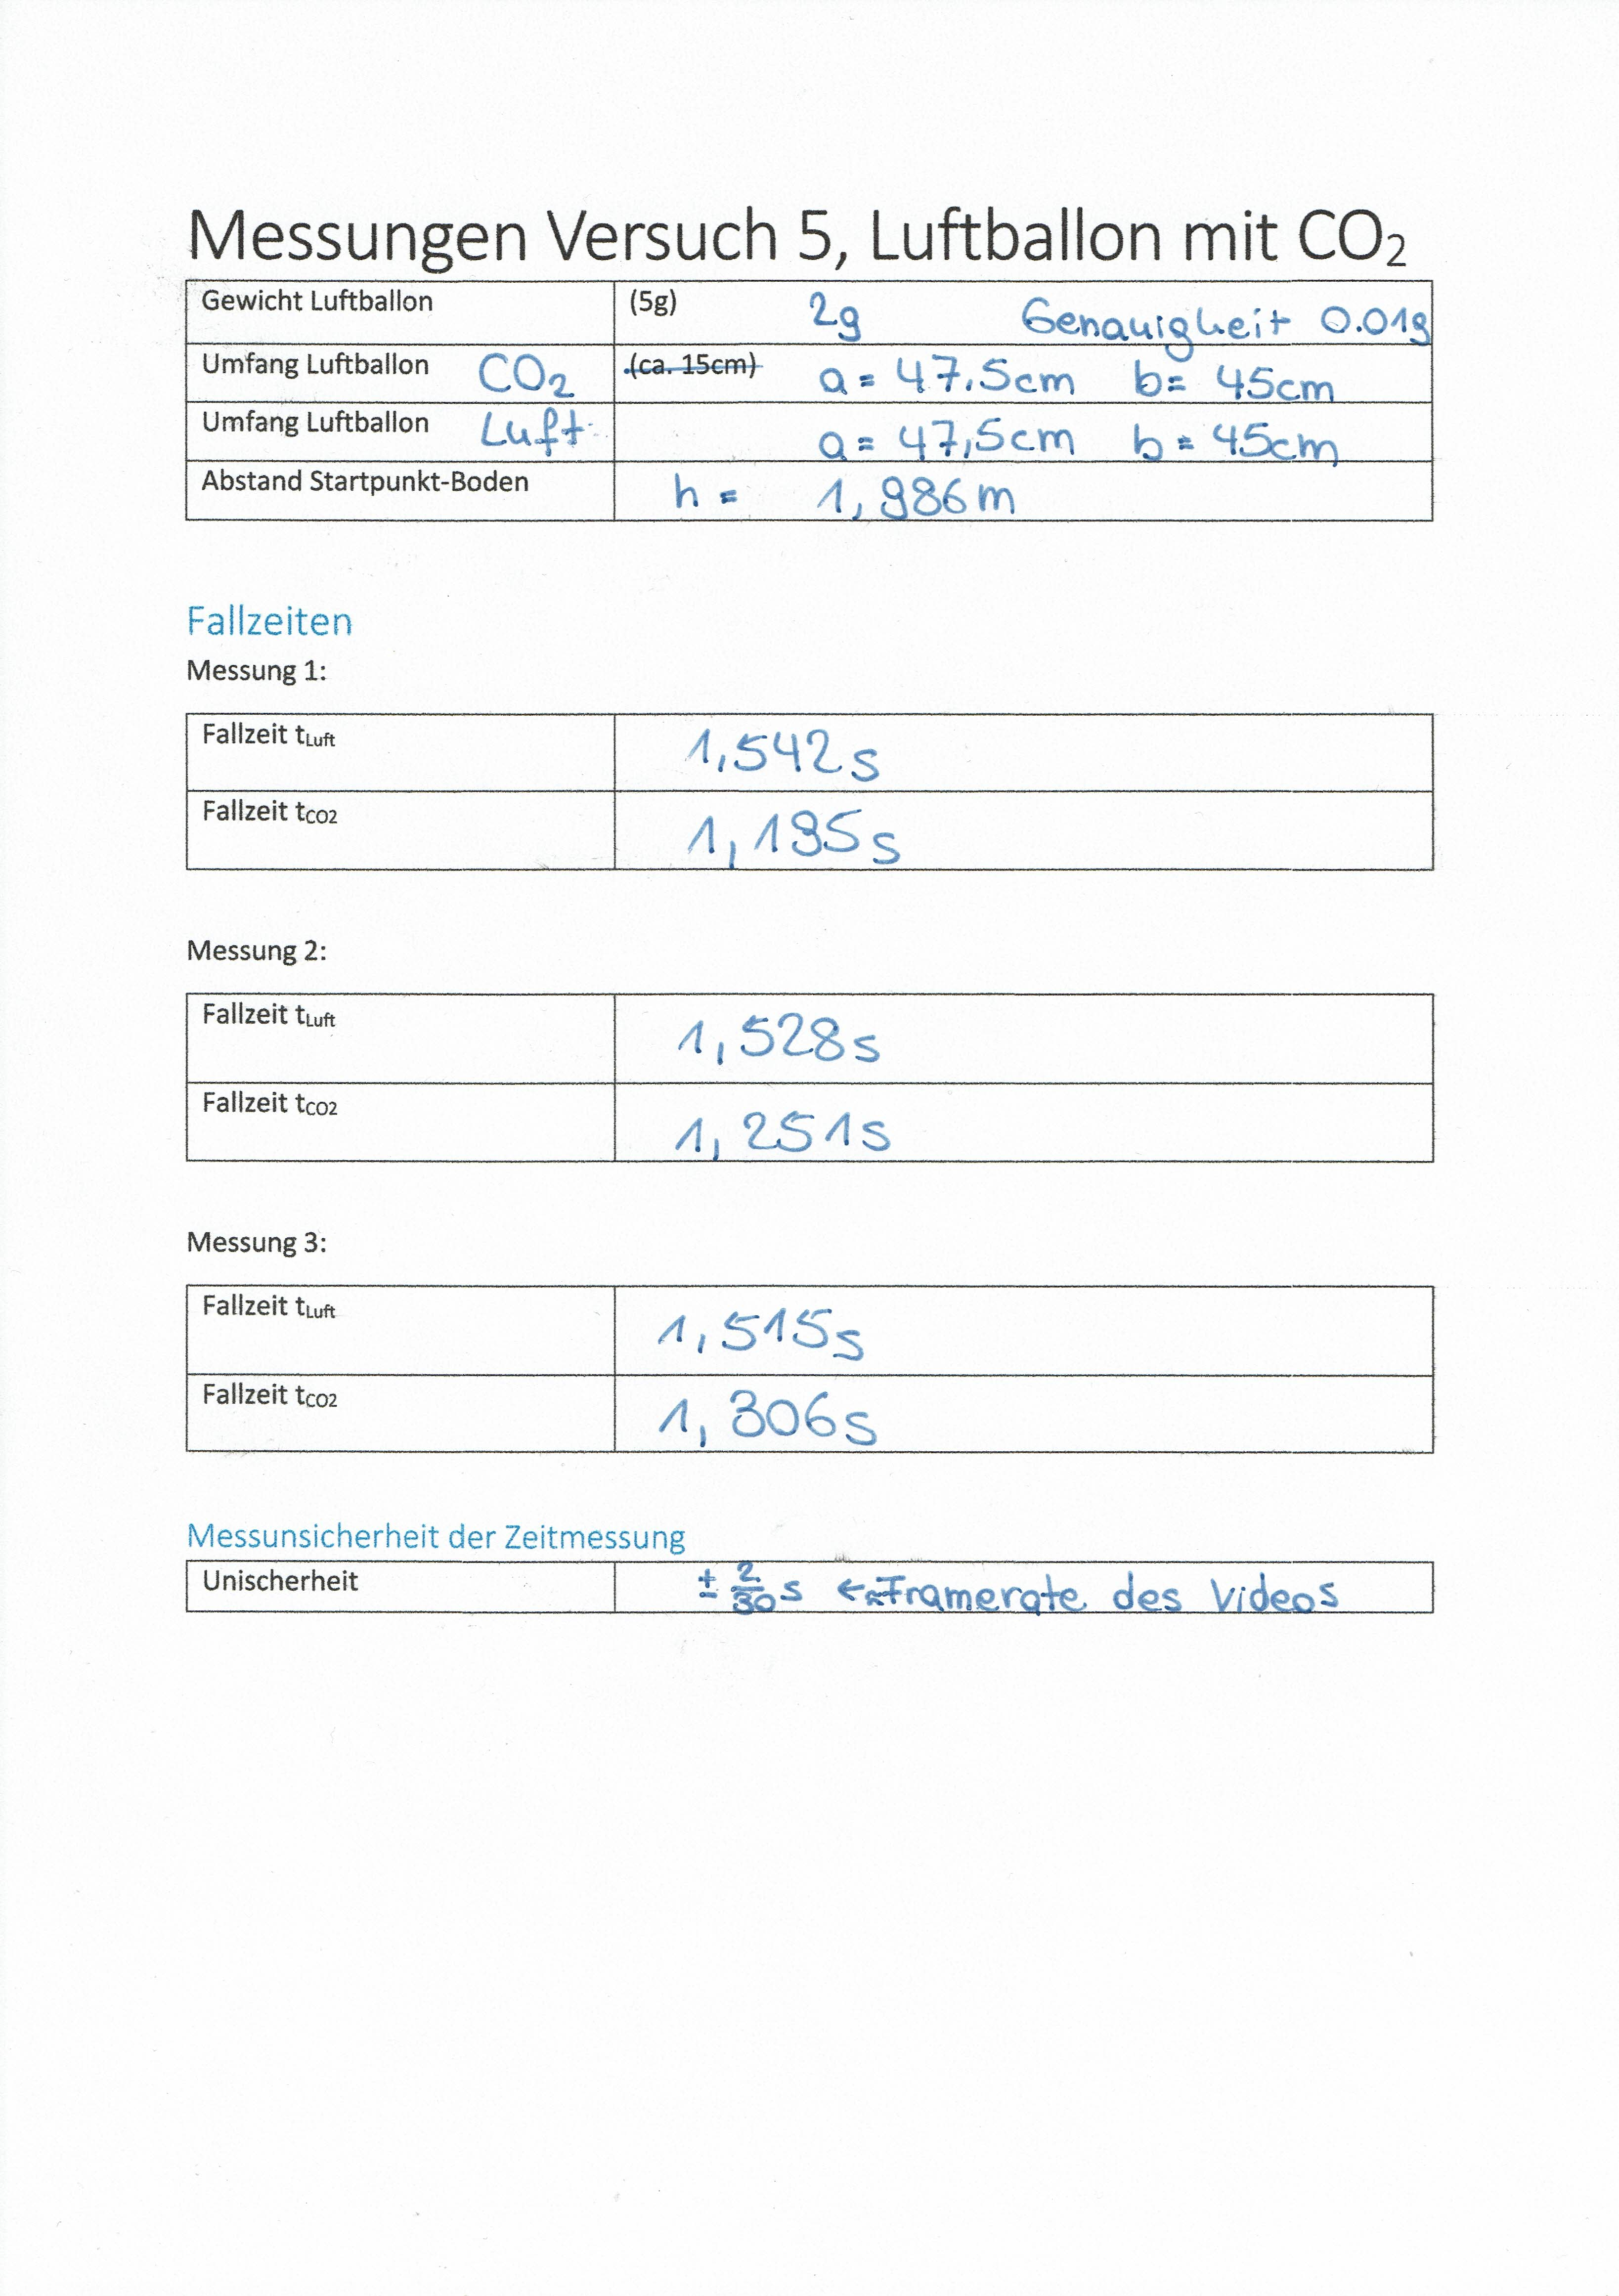
\includegraphics[height=14cm]{messwerte.jpg}
          \caption{Messwerte der drei Versuchsdurchführungen}
      \end{figure}

      \begin{figure}[ht]
          \centering
          \begin{minipage}[t]{0.4\textwidth}\label{fig:Fall2}
              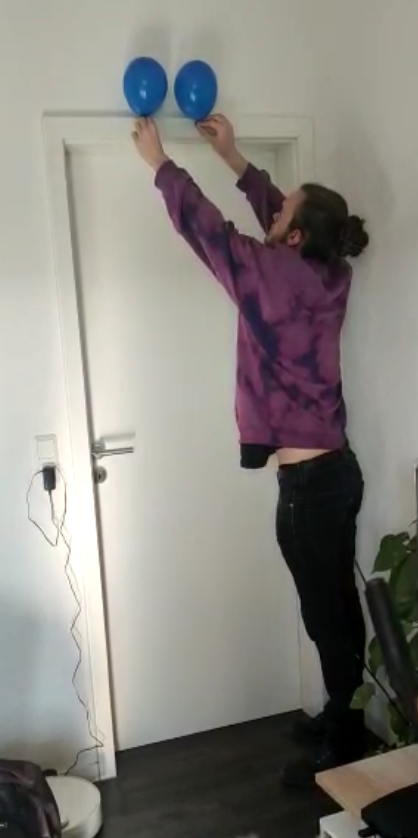
\includegraphics[height=14cm]{fallversuch2.png}
              \caption{Startposition der Versuchsdurchführung}
          \end{minipage}
          \hfill
          \begin{minipage}[t]{0.4\textwidth}\label{fig:Fall3}
              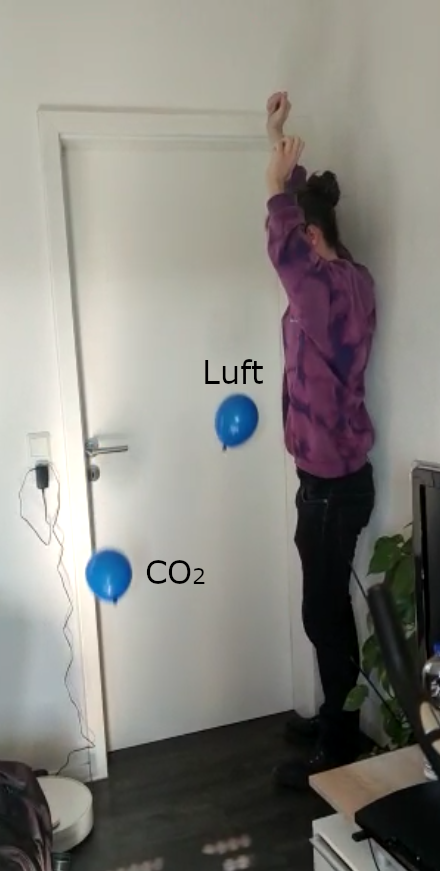
\includegraphics[height=14cm]{fallversuch3.png}
              \caption{Luftballons während dem Fall}
          \end{minipage}
      \end{figure}

\end{document}